\documentclass[14pt, compress, aspectratio=1610]{beamer}

\usetheme{pl}

\usepackage{longtable}
\usepackage{booktabs}
\usepackage{minted}
\usepackage{listings}
\usepackage{color}
\usepackage{fancyvrb}
\newcommand{\VerbBar}{|}
\newcommand{\VERB}{\Verb[commandchars=\\\{\}]}
\DefineVerbatimEnvironment{Highlighting}{Verbatim}{commandchars=\\\{\},fontsize=\small}
% Add ',fontsize=\small' for more characters per line
\usepackage[framemethod=tikz]{mdframed}
\definecolor{shadecolor}{HTML}{EEEEEE}
\mdfsetup{
  backgroundcolor=shadecolor,
  linecolor=shadecolor,
  innerleftmargin=5pt,
  innerrightmargin=5pt,
  leftmargin=-5pt,
  rightmargin=-5pt,
  roundcorner=3pt
}
\newenvironment{Shaded}{\begin{mdframed}}{\end{mdframed}}
\newcommand{\KeywordTok}[1]{\textcolor[rgb]{0.26,0.66,0.93}{\textbf{{#1}}}}
\newcommand{\DataTypeTok}[1]{\textcolor[rgb]{0.74,0.68,0.62}{\underline{{#1}}}}
\newcommand{\DecValTok}[1]{\textcolor[HTML]{558B2F}{{#1}}}
\newcommand{\BaseNTok}[1]{\textcolor[HTML]{558B2F}{{#1}}}
\newcommand{\FloatTok}[1]{\textcolor[HTML]{558B2F}{{#1}}}
\newcommand{\ConstantTok}[1]{\textcolor[rgb]{0.74,0.68,0.62}{{#1}}}
\newcommand{\CharTok}[1]{\textcolor[HTML]{7E57C2}{{#1}}}
\newcommand{\SpecialCharTok}[1]{\textcolor[HTML]{7E57C2}{{#1}}}
\newcommand{\StringTok}[1]{\textcolor[HTML]{7E57C2}{{#1}}}
\newcommand{\VerbatimStringTok}[1]{\textcolor[HTML]{7E57C2}{{#1}}}
\newcommand{\SpecialStringTok}[1]{\textcolor[HTML]{7E57C2}{{#1}}}
\newcommand{\ImportTok}[1]{\textcolor[rgb]{0.74,0.68,0.62}{{#1}}}
\newcommand{\CommentTok}[1]{\textcolor[HTML]{546E7A}{\textit{{#1}}}}
\newcommand{\DocumentationTok}[1]{\textcolor[HTML]{BCAAA4}{\textit{{#1}}}}
\newcommand{\AnnotationTok}[1]{\textcolor[HTML]{BCAAA4}{\textbf{\textit{{#1}}}}}
\newcommand{\CommentVarTok}[1]{\textcolor[rgb]{0.74,0.68,0.62}{{#1}}}
\newcommand{\OtherTok}[1]{\textcolor[rgb]{0.74,0.68,0.62}{{#1}}}
\newcommand{\FunctionTok}[1]{\textcolor[HTML]{26A69A}{\textbf{{#1}}}}
\newcommand{\VariableTok}[1]{\textcolor[rgb]{0.74,0.68,0.62}{{#1}}}
\newcommand{\ControlFlowTok}[1]{\textcolor[rgb]{0.26,0.66,0.93}{\textbf{{#1}}}}
\newcommand{\OperatorTok}[1]{\textcolor[rgb]{0.74,0.68,0.62}{{#1}}}
\newcommand{\BuiltInTok}[1]{\textcolor[HTML]{42A5F5}{{#1}}}
\newcommand{\ExtensionTok}[1]{\textcolor[rgb]{0.74,0.68,0.62}{{#1}}}
\newcommand{\PreprocessorTok}[1]{\textcolor[rgb]{0.74,0.68,0.62}{\textbf{{#1}}}}
\newcommand{\AttributeTok}[1]{\textcolor[rgb]{0.74,0.68,0.62}{{#1}}}
\newcommand{\RegionMarkerTok}[1]{\textcolor[rgb]{0.74,0.68,0.62}{{#1}}}
\newcommand{\InformationTok}[1]{\textcolor[rgb]{0.00,0.40,1.00}{\textbf{\textit{{#1}}}}}
\newcommand{\WarningTok}[1]{\textcolor[HTML]{FF6E40}{\textbf{{#1}}}}
\newcommand{\AlertTok}[1]{\textcolor[HTML]{FF3D00}{{#1}}}
\newcommand{\ErrorTok}[1]{\textcolor[HTML]{DD2C00}{\textbf{{#1}}}}
\newcommand{\NormalTok}[1]{\textcolor[HTML]{212121}{{#1}}}

% For adding citations/credits to slides
\newcommand{\btVFill}{\vskip0pt plus 1filll}
\newcommand{\credit}[1]{\btVFill\par\hfill \footnotesize ~#1}

\providecommand{\tightlist}{%
  \setlength{\itemsep}{0pt}\setlength{\parskip}{0pt}}

\let\OldTexttt\texttt
\renewcommand{\texttt}[1]{\OldTexttt{\color{plTT}#1}}

\makeatletter
\def\maxwidth{\ifdim\Gin@nat@width>\linewidth\linewidth\else\Gin@nat@width\fi}
\makeatother

\usepgfplotslibrary{dateplot}

\newcommand{\begincols}{\begin{columns}}
\newcommand{\stopcols}{\end{columns}}
\newcommand{\roundpicture}[2]{%
\tikz\node[circle,
          text=white,
          minimum width=4cm,
          minimum height=4cm,
          path picture={
              \node at (path picture bounding box.center){
                  \includegraphics[width=4cm]{#1}
              };
          }]{#2};
}
\newcommand{\plain}[1]{%
\begin{picture}(0,0)
  \put(-28.5,-175){%
      \pgfuseimage{titlebackground}
  }
  \put(0,-145){%
      \begin{minipage}[b][4.5cm][t]{0.5\textwidth}
          \color{white}\huge
              #1
      \end{minipage}
  }
\end{picture}
}

\title{Spatiotemporal forecasting of plant populations and the need to
partition forecast uncertainty}
\subtitle{}
\date{October 12, 2018}
\author{Andrew Tredennick}
\institute{University of Georgia}

\begin{document}

\maketitle

\begin{frame}{%
\protect\hypertarget{collaborators}{%
Collaborators}}

\(\phantom{testtesttt}\) Peter Adler (USU) \hspace{7em} Mevin Hooten
(CSU)

\(\phantom{testtest}\) \roundpicture{images/peter.jpg}{} \hspace{5em}
\roundpicture{images/mevin.jpg}{}

\end{frame}

\begin{frame}{%
\protect\hypertarget{rapid-environmental-change}{%
Rapid environmental change}}

\includegraphics[width=\textwidth]{./figures/mora_graphic.png}

\credit{Mora et al., 2013, \emph{Nature}}

\end{frame}

\begin{frame}{%
\protect\hypertarget{its-been-a-long-time-coming}{%
It’s been a long time coming}}

\includegraphics[width=\textwidth]{./figures/clark_title.pdf}

\credit{Clark et al., 2001, \emph{Science}}

\end{frame}

\begin{frame}{%
\protect\hypertarget{the-time-is-now}{%
The time is now}}

\includegraphics[width=\textwidth]{./figures/dietze_title.pdf}

\credit{Dietze et al., 2018, \emph{PNAS}}

\end{frame}

\begin{frame}{%
\protect\hypertarget{road-map}{%
Road map}}

\begin{enumerate}
[1.]
\tightlist
\item
  Do we need demographic data?
\item
  Scaling up plant population forecasts
\item
  Partitioning forecast uncertainty – a new agenda for ecology
\end{enumerate}

\end{frame}

\hypertarget{do-we-need-demographic-data}{%
\section{Do we need demographic
data?}\label{do-we-need-demographic-data}}

\begin{frame}{%
\protect\hypertarget{what-land-managers-want}{%
What land managers want}}

\centering

\includegraphics[height=2.7in]{./figures/managers_want.pdf}

\end{frame}

\begin{frame}{%
\protect\hypertarget{what-land-managers-get}{%
What land managers get}}

\centering

\includegraphics[height=2.8in]{./figures/managers_get.pdf}

\end{frame}

\begin{frame}{%
\protect\hypertarget{really-hard-work}{%
Really hard work}}

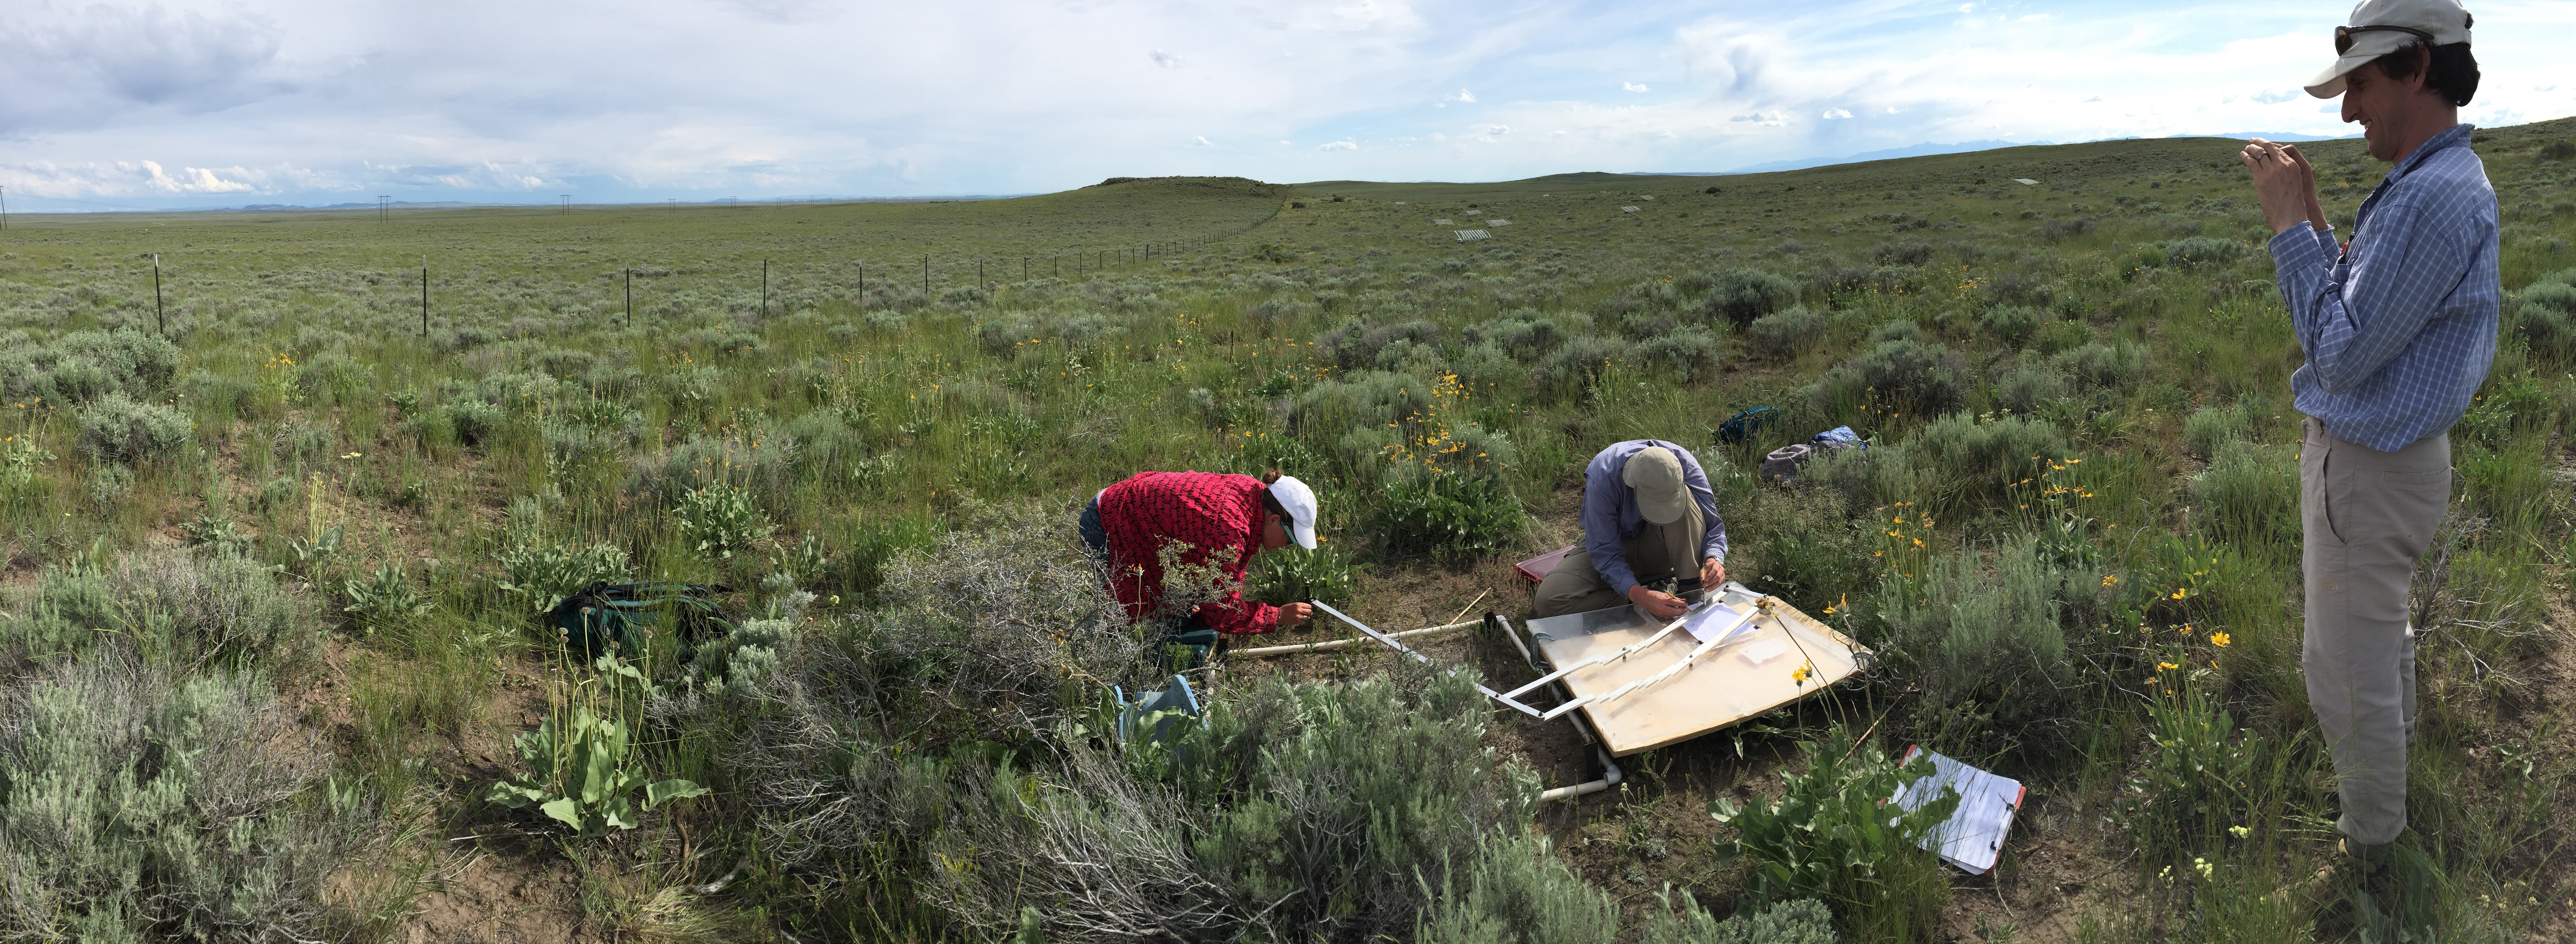
\includegraphics[width=\textwidth]{./figures/chart_measuring.jpg}

\end{frame}

\begin{frame}{%
\protect\hypertarget{aggregate-population-level-data}{%
Aggregate population-level data}}

\includegraphics[width=\textwidth]{./figures/missing_climate.pdf}

\end{frame}

\begin{frame}{%
\protect\hypertarget{objectives}{%
Objectives}}

\begin{enumerate}
[1.]
\tightlist
\item
  Determine if population-level data contains similar climate signal as
  individual-level data.
\item
  Compare model accuracy and precision using out-of-sample validation.
\end{enumerate}

\end{frame}

\begin{frame}{%
\protect\hypertarget{year-time-series-from-montana}{%
14-year time series from Montana}}

\includegraphics[width=\textwidth]{./figures/mt_spp.png}

\end{frame}

\begin{frame}{%
\protect\hypertarget{two-types-of-models}{%
Two types of models}}

\centering

\includegraphics[height=2.7in]{./figures/mee_flow.png}

\end{frame}

\begin{frame}{%
\protect\hypertarget{integral-projection-model}{%
Integral projection model}}

\centering

\includegraphics[width=0.7\textwidth]{./figures/maps.pdf}

\begin{align*}
\text{survival}(t+1) &\phantom{=} \\
\text{growth}(t+1) &= f\left(\text{size}(t),\text{location},\text{crowding}(t),\text{year}(t),\text{climate}(t) \right) \\
\text{recruitment}(t+1) &\phantom{=} \\
\end{align*}

\end{frame}

\begin{frame}{%
\protect\hypertarget{qaudratcover-based-model}{%
Qaudrat(cover)-based model}}

\includegraphics[width=\textwidth]{./figures/montana_quad_ts.pdf}

\[
\text{cover}(t+1) = f\left(\text{cover}(t),\text{location},\text{year}(t),\text{climate}(t) \right)
\]

\end{frame}

\begin{frame}{%
\protect\hypertarget{climate-covariates}{%
Climate covariates}}

\includegraphics[width=\textwidth]{./figures/ipm_climate_effects.pdf}

\end{frame}

\begin{frame}{%
\protect\hypertarget{climate-effects-by-vital-rates}{%
Climate effects by vital rates}}

\centering

\includegraphics[height=2.5in]{./figures/mee_climate_effects.pdf}

\credit{Tredennick et al., 2017, \emph{Methods in Ecol. Evol.}}

\end{frame}

\begin{frame}{%
\protect\hypertarget{model-comparison}{%
Model comparison}}

\centering

\includegraphics[height=2.5in]{./figures/mee_forecast_accuracy_empty.pdf}

\credit{Tredennick et al., 2017, \emph{Methods in Ecol. Evol.}}

\end{frame}

\begin{frame}{%
\protect\hypertarget{model-comparison-1}{%
Model comparison}}

\centering

\includegraphics[height=2.5in]{./figures/mee_forecast_accuracy.pdf}

\credit{Tredennick et al., 2017, \emph{Methods in Ecol. Evol.}}

\end{frame}

\begin{frame}{%
\protect\hypertarget{forecast-horizons}{%
Forecast horizons}}

\centering

\includegraphics[height=2.5in]{./figures/mee_horizons.pdf}

\credit{Tredennick et al., 2017, \emph{Methods in Ecol. Evol.}}

\end{frame}

\begin{frame}{%
\protect\hypertarget{do-we-need-demographic-data-1}{%
Do we need demographic data?}}

\centering

Maybe not.

\end{frame}

\hypertarget{scaling-up-plant-population-forecasts}{%
\section{Scaling up plant population
forecasts}\label{scaling-up-plant-population-forecasts}}

\begin{frame}{%
\protect\hypertarget{sagebrush-sea-in-wyoming}{%
Sagebrush sea in Wyoming}}

\centering

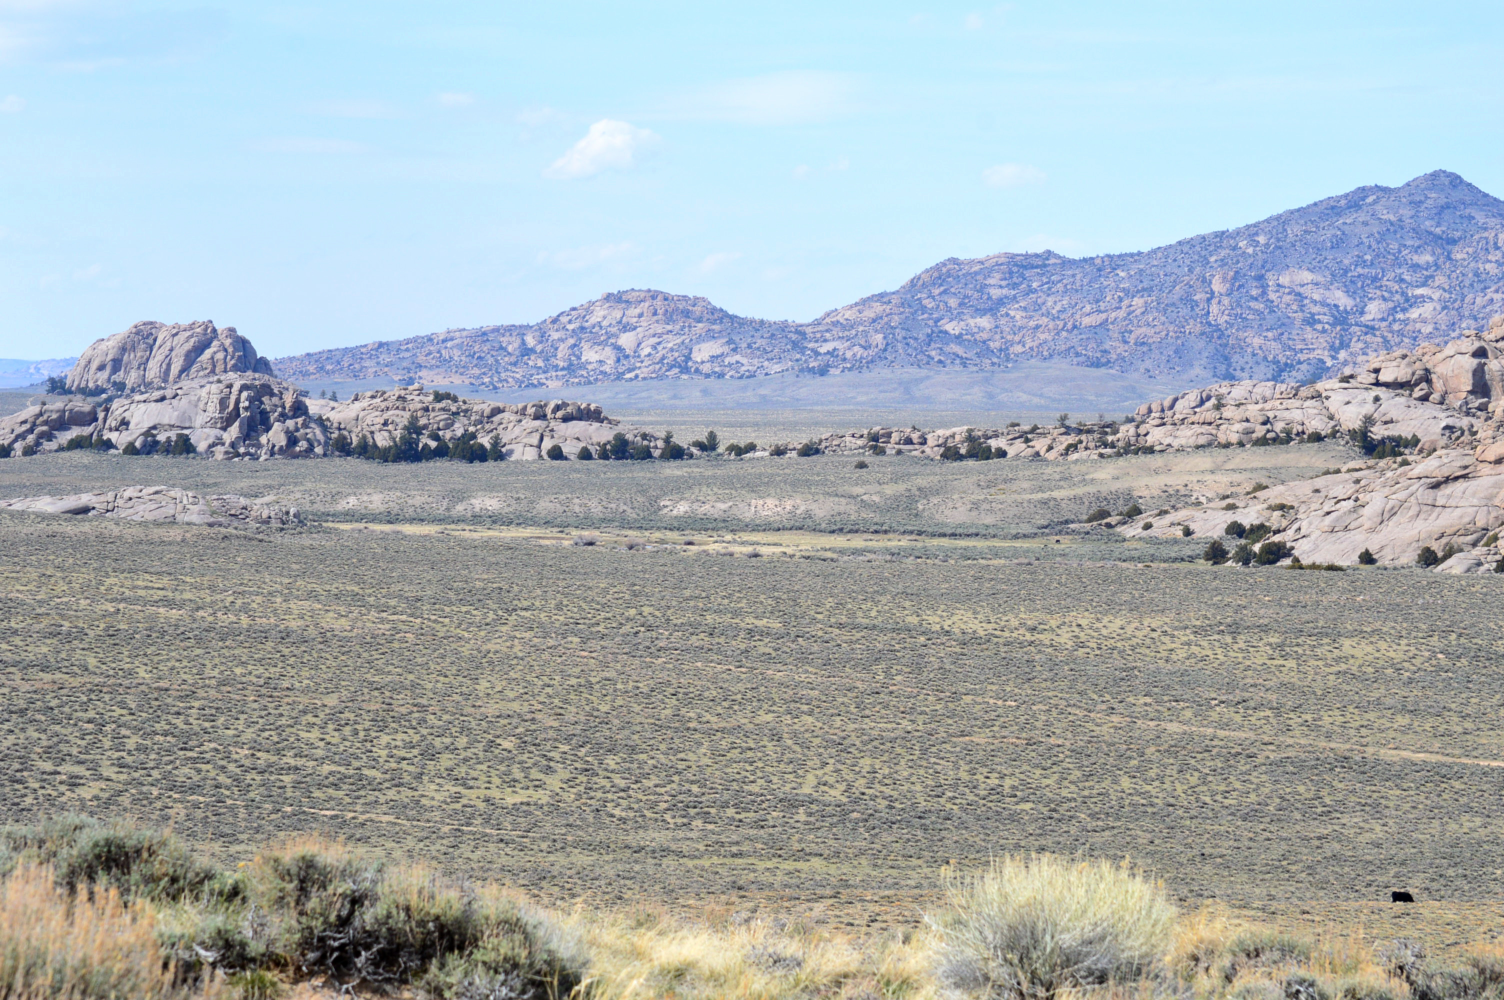
\includegraphics[height=2.5in]{./figures/sage_pic.pdf}

\end{frame}

\begin{frame}{%
\protect\hypertarget{study-area}{%
Study area}}

\centering

\includegraphics[height=2.8in]{./figures/studyarea_map.png}

\end{frame}

\begin{frame}{%
\protect\hypertarget{landsat-time-series}{%
Landsat time series}}

\includegraphics[height=2.8in]{./figures/all_years_percCover.pdf}

\end{frame}

\begin{frame}{%
\protect\hypertarget{dynamic-cover-model}{%
Dynamic cover model}}

\begin{align*}
y_{i,t} &\sim \text{Poisson}(\mu_{i,t}) \\
\text{log}(\mu_{i,t}) &= \underbrace{\beta_{0,t} + \beta_{1}y_{i,t-1}}_\text{temporal + dens. dep} + \underbrace{\textbf{x}_{t}'\boldsymbol{\phi}}_\text{climate} + \underbrace{\eta_{i}}_\text{spatial}
\end{align*}

\end{frame}

\begin{frame}{%
\protect\hypertarget{dimension-reduction-for-spatial-effect}{%
Dimension reduction for spatial effect}}

\includegraphics[width=\textwidth]{./figures/SAGE_Grid_wKnots_subset.png}

\end{frame}

\begin{frame}{%
\protect\hypertarget{dynamic-cover-model-1}{%
Dynamic cover model}}

\begin{align*}
y_{i,t} &\sim \text{Poisson}(\mu_{i,t}) \\
\text{log}(\mu_{i,t}) &= \underbrace{\beta_{0,t} + \beta_{1}y_{i,t-1}}_\text{temporal + dens. dep} + \underbrace{\textbf{x}_{t}'\boldsymbol{\phi}}_\text{climate} + \underbrace{\eta_{i}}_\text{spatial} \\
\boldsymbol{\eta} &\approx \textbf{K}\boldsymbol{\alpha}, \\
\alpha_{m} &\sim \text{Normal}(0,\sigma_{\eta}^2)
\end{align*}

\end{frame}

\begin{frame}{%
\protect\hypertarget{climate-effects}{%
Climate effects}}

\centering

\includegraphics[height=2.7in]{./figures/post_climate_covariates.pdf}

\end{frame}

\begin{frame}{%
\protect\hypertarget{model-performance}

\includegraphics[width=\textwidth]{./figures/obs_predict_spatial_pres.pdf}

\credit{Tredennick et al., 2016, \emph{Ecosphere}}

\end{frame}

\begin{frame}{%
\protect\hypertarget{forecasts-under-climate-change-spatial}{%
Forecasts under climate change: spatial}}

\includegraphics[width=\textwidth]{./figures/clim_change_mean_spatial_empty.pdf}

\credit{Tredennick et al., 2016, \emph{Ecosphere}}

\end{frame}

\begin{frame}{%
\protect\hypertarget{forecasts-under-climate-change-spatial-1}{%
Forecasts under climate change: spatial}}

\includegraphics[width=\textwidth]{./figures/clim_change_mean_spatial.pdf}

\credit{Tredennick et al., 2016, \emph{Ecosphere}}

\end{frame}

\begin{frame}{%
\protect\hypertarget{forecasts-under-climate-change-temporal}{%
Forecasts under climate change: temporal}}

\centering

\includegraphics[height=2in]{./figures/temporal_forecasts_presentation.pdf}

\credit{Tredennick et al., 2016, \emph{Ecosphere}}

\end{frame}

\hypertarget{partitioning-forecast-uncertainty}{%
\section{Partitioning forecast
uncertainty}\label{partitioning-forecast-uncertainty}}

\begin{frame}{%
\protect\hypertarget{forecast-varianceto-a-first-approximation}{%
Forecast variance\ldots{}to a first approximation}}

\[
y_{t+1} = f(y_t, x_t|\theta) + \epsilon_{t+1}
\]

\end{frame}

\begin{frame}{%
\protect\hypertarget{forecast-varianceto-a-first-approximation-1}{%
Forecast variance\ldots{}to a first approximation}}

\[
y_{t+1} = f(y_t, x_t|\theta) + \epsilon_{t+1}
\]

\small\begin{align*}
Var[y_{t+1}] \approx \underbrace{\left(\frac{\delta f}{\delta y} \right)^2}_{\text{stability}} 
               \underbrace{\vphantom{ \left(\frac{\delta f}{\delta y} \right)^2 } Var[y_t]}_{\text{IC uncert.}} +
               \underbrace{\vphantom{ \left(\frac{\delta f}{\delta y} \right)^2 }\left(\frac{\delta f}{\delta x} \right)^2}_{\text{driver sens.}} 
               \underbrace{\vphantom{ \left(\frac{\delta f}{\delta y} \right)^2 } Var[x_t]}_{\text{driver uncert.}} +
               \underbrace{\vphantom{ \left(\frac{\delta f}{\delta y} \right)^2 }\left(\frac{\delta f}{\delta \theta} \right)^2}_{\text{param sens.}}
               \underbrace{\vphantom{ \left(\frac{\delta f}{\delta y} \right)^2 } Var[\theta]}_{\text{param. uncert.}} +
               \underbrace{\vphantom{ \left(\frac{\delta f}{\delta y} \right)^2 } Var[\epsilon]}_{\text{process error}}
\end{align*}

\credit{Dietze, 2017, \emph{Ecological Applications}; Cariboni et al., 2007, \emph{Ecological Modeling}}

\end{frame}

\begin{frame}{%
\protect\hypertarget{forecast-varianceto-a-first-approximation-2}{%
Forecast variance\ldots{}to a first approximation}}

\colorlet{shadecolor}{gray!40}

\[
\textcolor{shadecolor}{y_{t+1} = f(y_t, x_t|\theta) + \epsilon_{t+1}}
\]

\small\begin{align*}
\textcolor{shadecolor}{Var[y_{t+1}] \approx \underbrace{\left(\frac{\delta f}{\delta y} \right)^2}_{\text{stability}} 
               \underbrace{\vphantom{ \left(\frac{\delta f}{\delta y} \right)^2 } Var[y_t]}_{\text{IC uncert.}} +
               \underbrace{\vphantom{ \left(\frac{\delta f}{\delta y} \right)^2 }\left(\frac{\delta f}{\delta x} \right)^2}_{\text{driver sens.}} 
               \underbrace{\vphantom{ \left(\frac{\delta f}{\delta y} \right)^2 } Var[x_t]}_{\text{driver uncert.}} +
               \underbrace{\vphantom{ \left(\frac{\delta f}{\delta y} \right)^2 }\left(\frac{\delta f}{\delta \theta} \right)^2}_{\text{param sens.}}
               \underbrace{\vphantom{ \left(\frac{\delta f}{\delta y} \right)^2 } Var[\theta]}_{\text{param. uncert.}} +
               \underbrace{\vphantom{ \left(\frac{\delta f}{\delta y} \right)^2 } Var[\epsilon]}_{\text{process error}}}
\end{align*}

\normalsize

\[
Var[y_{t+1}] \approx \text{Internal}+\text{External}+\text{Parameters}+\text{Process Error}
\]

\credit{Dietze, 2017, \emph{Ecological Applications}; Cariboni et al., 2007, \emph{Ecological Modeling}}

\end{frame}

\begin{frame}{%
\protect\hypertarget{this-is-why-we-have-weather-satellites}{%
This is why we have weather satellites}}

\begincols\column{0.68\textwidth}

\begin{align*}
Var[y_{t+1}] \approx \underbrace{\left(\frac{\delta f}{\delta y} \right)^2}_{\text{stability}} 
               \underbrace{\vphantom{ \left(\frac{\delta f}{\delta y} \right)^2 } Var[y_t]}_{\text{IC uncert.}} 
\end{align*}

\[
Var[y_{t+1}] \approx \text{Internal}
\]

\hfill\column{0.28\textwidth}

\roundpicture{figures/satellite.jpg}{}

\stopcols

\end{frame}

\begin{frame}{%
\protect\hypertarget{yellowstone-bison-bison-bison}{%
Yellowstone bison (\emph{Bison bison})}}

\includegraphics[width=\textwidth]{./figures/National-Park_Sandy-Sist.jpg}

\end{frame}

\begin{frame}{%
\protect\hypertarget{yellowstone-bison-bison-bison-1}{%
Yellowstone bison (\emph{Bison bison})}}

\centering

\includegraphics[height=2.7in]{./figures/bison_winter.jpg}

\end{frame}

\begin{frame}{%
\protect\hypertarget{time-series-of-bison-counts-1970---2017}{%
Time series of bison counts (1970 - 2017)}}

\begin{description}
\tightlist
\item[Response]
Bison counts
\item[Covariate]
January precipitation
\end{description}

\includegraphics[width=\textwidth]{./figures/bison_data_plots.png}

\end{frame}

\begin{frame}{%
\protect\hypertarget{gompertz-population-growth}{%
Gompertz population growth}}

\begin{align*}
mu_{(t)} &= \text{log}(z_{(t-1)}) + e_{(t)} + r + b_0 \text{log}(z_{(t-1)} + e_{(t)}) + b_1 x_{(t)} \\
\text{log}(z_{(t)}) &\sim \text{Normal}\left( \mu_{(t)}, \sigma^2_\text{p} \right)
\end{align*}

\footnotesize

\begin{description}
\tightlist
\item[\(z_t\)]
\alert{latent} population abundance in year \emph{t}
\item[\(e_t\)]
log of harvested animals between \(t-1\) and \(t\)
\item[\(r\)]
per capita growth rate
\item[\(b_0\)]
density dependence
\item[\(b_1\)]
effect of January precipitation
\item[\(x_t\)]
January precipitation in year \emph{t}
\item[\(\sigma^2_\text{p}\)]
process variance
\end{description}

\end{frame}

\begin{frame}{%
\protect\hypertarget{likelihood-and-fully-specified-model}{%
Likelihood and fully specified model}}

Likelihood

\[
 y_{(t)} \sim \text{NB} \left(  z_{(t)} , \kappa \right)
 \]

Full model

\small

\[
 \left[ \boldsymbol{\theta}_\text{p}, \kappa, z_{(t)}, z_{(t-1)} | y_{(t)}, x_{(t)} \right ] \propto \prod_{t=2}^{\textcolor{red}{48}} \underbrace{\left[ z_{(t)} | \boldsymbol{\theta}_\text{p}, z_{(t-1)}, x_{(t)} \right]}_{\text{process}} \prod_{t=1}^{\textcolor{red}{41}} \underbrace{\left[ y_{(t)} | \kappa, z_{(t)} \right]}_{\text{data}} \underbrace{\left[ \boldsymbol{\theta}_\text{p}, \kappa, z_{(t=1)}\right]}_{\text{parameters}}
 \]

\end{frame}

\begin{frame}{%
\protect\hypertarget{posterior-distribution-of-climate-effect}{%
Posterior distribution of climate effect}}

\centering

\includegraphics[height = 2.5in]{./figures/bison_post_params.pdf}

\end{frame}

\begin{frame}{%
\protect\hypertarget{model-fit-and-forecast}{%
Model fit and forecast}}

\centering

\includegraphics[height=2.7in]{./figures/bison_fit.pdf}

\end{frame}

\begin{frame}{%
\protect\hypertarget{forecast-partition}{%
Forecast partition}}

\centering

\includegraphics[height=2.7in]{./figures/forecast_partition.pdf}

\end{frame}

\begin{frame}{%
\protect\hypertarget{climate-projections-are-uncertain}{%
Climate Projections are uncertain}}

\centering

\includegraphics[height=2.7in]{./figures/precip_projections.pdf}

\end{frame}

\hypertarget{closing-thoughts}{%
\section{Closing thoughts}\label{closing-thoughts}}

\begin{frame}{%
\protect\hypertarget{closing-thoughts-1}{%
Closing thoughts}}

\begin{enumerate}
[1.]
\tightlist
\item
  We have the tools and the data streams to start forecasting.
\item
  The time to start is now.
\item
  Embrace our failures.
\item
  Generate \alert{meaningful} forecasts – forecasts that someone wants.
\end{enumerate}

\end{frame}

\begin{frame}[plain]
  \begin{picture}(0,0)
    \put(-28.5,-175){%
      \pgfuseimage{titlebackground}
    }
  \end{picture}
\end{frame}

\end{document}
